\chapter{Lab Lock:锁的实验}
\begin{introduction}
    \item 实现每个 CPU 独占的内存分配器
    \item 实现 IO 缓存
    \item 减少加锁开销
\end{introduction}

前面的很多实验中都涉及到了加锁的问题。锁作为一种互斥机制,对于开发者而言实现简单,理解其行为也不复杂,且能提供可靠的互斥保障。但过多的加锁操作会显著地降低系统的并行性,从而使得多处理机系统无法发挥其应有的性能。本部分实验中,主要涉及对于加锁机制的优化,从而增加 xv6 内核的并行性。

\section{实现每个 CPU 独占的内存分配器}

在这个实验中, xv6 提供了用户态程序 \lstinline{kalloctest} ,用于对 xv6 的内存分配器进行压力测试。用户态程序 \lstinline{kalloctest} 产生三个进程,这些进程会不断分配并释放内存,使得原始的 xv6 中的只有一个空闲链表的数据结构的锁被不断获取和释放,且大多数时候对锁的 \lstinline{acquire()} 会被阻塞。用户态程序 \lstinline{kalloctest} 会统计 \lstinline{acquire()} 时被阻塞消耗的循环次数,用以估计加锁产生的额外开销。

在我们没有改进 xv6 的内存分配器之前,编译并运行 xv6 ,然后运行 \lstinline{kalloctest} ,会得到类似下面的结果:
\begin{lstlisting}
    $ kalloctest
    start test1
    test1 results:
    --- lock kmem/bcache stats
    lock: kmem: #fetch-and-add 83375 #acquire() 433015
    lock: bcache: #fetch-and-add 0 #acquire() 1260
    --- top 5 contended locks:
    lock: kmem: #fetch-and-add 83375 #acquire() 433015
    lock: proc: #fetch-and-add 23737 #acquire() 130718
    lock: virtio_disk: #fetch-and-add 11159 #acquire() 114
    lock: proc: #fetch-and-add 5937 #acquire() 130786
    lock: proc: #fetch-and-add 4080 #acquire() 130786
    tot= 83375
    test1 FAIL
\end{lstlisting}

可见 \lstinline{acquire()} 时被阻塞消耗的循环的计数十分巨大,说明内存分配时等待获取锁会浪费大量时间,从而使得内存分配的效率较低。

根据 xv6 手册的提示,一种降低加锁引起的开销的方法是为每一个 CPU 核心设置一个单独的空闲链表和对应的锁,这样运行在某 CPU 上的进程在试图分配内存时,会获取自己所在的 CPU 上空闲链表的锁然后尝试分配内存,只有当无法分配内存时,内存分配器才会到其它 CPU 的空闲链表中借取空闲的页面。

\begin{proposition}[资源重复设置与减小加锁开销] 
    从另一个角度看,这里为每个 CPU 设置一个内存分配器属于资源的重复设置。通过重复设置资源,可以使得进程直接获得锁而无需等待的概率大大提高,从而降低了进程等待时间的期望值,故整个系统的效率能够得到提高。但是,资源重复设置可能会引起诸如数据一致性等问题,故而会大大增加软件的复杂度。
\end{proposition}

首先,我们修改 \lstinline{kalloc.c} 中的数据结构,使单一的空闲链表变为多个空闲链表的数组:
\begin{lstlisting}[language=C]
    struct {
        struct spinlock lock;
        struct run *freelist;
      } kmem[NCPU];
\end{lstlisting}

然后,我们需要根据上面的分配与释放的逻辑,对 \lstinline{kalloc()} 进行修改。首先需要利用 \lstinline{cpuid()} 读取特殊寄存器以获得当前运行的 CPU 的编号,该编号对应着一个空闲链表,在获取该编号时需要关闭中断,以免发生不测。
\begin{lstlisting}[language=C]
void *
kalloc(void)
{
  struct run *r;
  push_off();
  int c = cpuid();
  pop_off();
......
\end{lstlisting}

成功获取 CPU 编号后,我们需要获取对应的空闲链表的锁,然后试图分配页面:
\begin{lstlisting}[language=C]
......
  acquire(&kmem[c].lock);
  r = kmem[c].freelist;
  if(r)
  {
    kmem[c].freelist = r->next;
    release(&kmem[c].lock);
......
\end{lstlisting}

若该 CPU 的空闲链表中没有空闲页面,则到其它 CPU 中借用一个:
\begin{lstlisting}[language=C]
......
} else {
    release(&kmem[c].lock);
    for (int i = 0; i<NCPU; i++)
    {
      acquire(&kmem[i].lock);
      r = kmem[i].freelist;
      if(r)
      {
        kmem[i].freelist = r->next;
        release(&kmem[i].lock);
        break;
      } else {
        release(&kmem[i].lock);
      }
    }
  }
......
\end{lstlisting}

最后若分配成功,则返回获取的页面,笔者完整的实现如下:
\begin{lstlisting}[language=C]
void *
kalloc(void)
{
  struct run *r;
  push_off();
  int c = cpuid();
  pop_off();

  acquire(&kmem[c].lock);
  r = kmem[c].freelist;
  if(r)
  {
    kmem[c].freelist = r->next;
    release(&kmem[c].lock);
  } else {
    release(&kmem[c].lock);
    for (int i = 0; i<NCPU; i++)
    {
      acquire(&kmem[i].lock);
      r = kmem[i].freelist;
      if(r)
      {
        kmem[i].freelist = r->next;
        release(&kmem[i].lock);
        break;
      } else {
        release(&kmem[i].lock);
      }
    }
  }
  if(r)
    memset((char*)r, 5, PGSIZE);  // fill with junk
  return (void*)r;
}
\end{lstlisting}

对分配内存的 \lstinline{kalloc()} 修改完成后,我们还需要修改对应的用于释放内存的 \lstinline{kfree()} ,直接将页面加入到当前的 CPU 空闲链表中(即便是借来的页面,也不归还了),实现如下:
\begin{lstlisting}[language=C]
void
kfree(void *pa)
{
  struct run *r;
  push_off();
  int c = cpuid();
  pop_off();

  if(((uint64)pa % PGSIZE) != 0 || (char*)pa < end || (uint64)pa >= PHYSTOP)
    panic("kfree");

  // Fill with junk to catch dangling refs.
  memset(pa, 1, PGSIZE);

  r = (struct run*)pa;

  acquire(&kmem[c].lock);
  r->next = kmem[c].freelist;
  kmem[c].freelist = r;
  release(&kmem[c].lock);
}
\end{lstlisting}

最后不要忘记初始化内存分配器的 \lstinline{kinit()} ,其需要初始化每个 CPU 的空闲链表和锁:
\begin{lstlisting}[language=C]
void
kinit()
{
  for (int i = 0; i<NCPU; i++)
  {
    initlock(&kmem[i].lock, "kmem");
  }
  freerange(end, (void*)PHYSTOP);
}
\end{lstlisting}

调用 \lstinline{freerange} 的 CPU 会在初始化时获得所有的空闲页面,不过无需担心分配不均,这些页面会在一次次的 \lstinline{kalloc()} 和 \lstinline{kfree()} 的过程中进入其它 CPU 的空闲链表中。

至此,对于 xv6 的内存分配器的改造已经完成,再次编译并运行 xv6 ,然后运行 \lstinline{kalloctest} ,会得到类似下图的结果:
\begin{figure}[H]
  \centering
  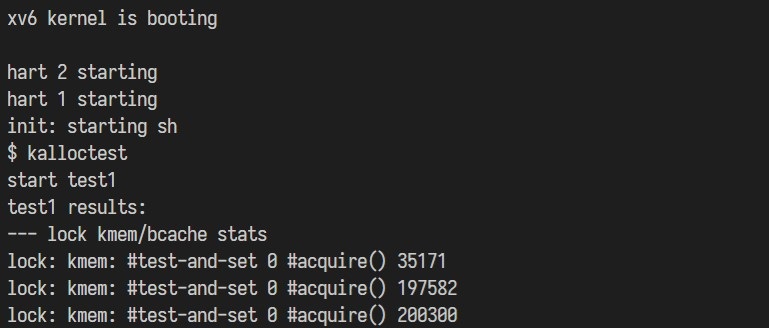
\includegraphics[width=0.8\textwidth]{lock_kalloctest.jpg}
  \caption{ \lstinline{kalloctest} 的测试结果}
\end{figure}
最后 \lstinline{kalloctest} 输出 \lstinline{test0 OK} 、 \lstinline{test1 OK} 和 \lstinline{test2 OK},且加锁开销远小于改进前的值,符合我们的预期。

\section{实现 IO 缓存}

由于磁盘等外存设备普遍读写速度较慢,故很多操作系统都会在其文件系统的机制中设置外存块的缓存,以提高整个系统的性能。在 xv6 中也有类似的机制,在 \lstinline{bio.c} 中可以看到其实现。

在原始的 xv6 中,对于缓存的读写是由单一的锁 \lstinline{bcache.lock} 来保护的,这就导致了如果系统中有多个进程在进行 IO 操作,则等待获取 \lstinline{bcache.lock} 的开销就会较大。为了减少加锁的开销, xv6 的实验手册提示我们可以将缓存分为几个桶,为每个同单独设置一个锁,这样如果两个进程访问的缓存块在不同的桶中,则可以同时获得两个锁从而进行操作,而无需等待加锁。我们的目标是将 \lstinline{bcachetest} 中统计值 \lstinline{tot} 降到规定值以下,在没有改进前, xv6 中运行 \lstinline{bcachetest} 的结果大致如下:
\begin{lstlisting}
    $ bcachetest
    start test0
    test0 results:
    --- lock kmem/bcache stats
    lock: kmem: #fetch-and-add 0 #acquire() 33035
    lock: bcache: #fetch-and-add 16142 #acquire() 65978
    --- top 5 contended locks:
    lock: virtio_disk: #fetch-and-add 162870 #acquire() 1188
    lock: proc: #fetch-and-add 51936 #acquire() 73732
    lock: bcache: #fetch-and-add 16142 #acquire() 65978
    lock: uart: #fetch-and-add 7505 #acquire() 117
    lock: proc: #fetch-and-add 6937 #acquire() 73420
    tot= 16142
    test0: FAIL
    start test1
    test1 OK
\end{lstlisting}


依照上面的思想,我们首先改造 \lstinline{bcache} 的数据结构,将单个锁改成多个锁,并将缓存块分组:
\begin{lstlisting}[language=C]
    struct {
        struct spinlock lock[NBUCKET];
        struct buf buf[NBUF];

        struct buf bucket[NBUCKET];
      } bcache;
\end{lstlisting}

然后,修改对应的一些头文件中的定义,如在 \lstinline{param.h} 中:
\begin{lstlisting}[language=C]
    #define NBUF         (MAXOPBLOCKS*12)  // size of disk block cache
\end{lstlisting}
在 \lstinline{defs.h} 中:
\begin{lstlisting}[language=C]
    int             can_lock(int, int);
\end{lstlisting}

在 \lstinline{buf.h} 中:
\begin{lstlisting}[language=C]
    struct buf {
        int valid;   // has data been read from disk?
        int disk;    // does disk "own" buf?
        uint dev;
        uint blockno;
        struct sleeplock lock;
        uint refcnt;
        struct buf *prev; // LRU cache list
        struct buf *next;
        uchar data[BSIZE];
        uint time;
      };
\end{lstlisting}

然后,修改对应的 \lstinline{bcache} 初始化函数 \lstinline{binit()} ,使之与修改后的数据结构相适应:
\begin{lstlisting}[language=C]
void binit(void)
{
  struct buf *b;

  for (int i = 0; i < NBUCKET; i++)
  {
    initlock(&bcache.lock[i], "bcache.bucket");
  }
  b = &bcache.bucket[0];
  for (int i = 0; i < NBUF; i++)
  {
    b->next = &bcache.buf[i];
    b = b->next;
    initsleeplock(&b->lock, "buffer");
  }
}
\end{lstlisting}

之后构建一个辅助函数 \lstinline{can_lock()} ,用于避免死锁:
\begin{lstlisting}[language=C]
int can_lock(int cur_idx, int req_idx)
{
  int mid = NBUCKET / 2;
  // non-reentrant
  if (cur_idx == req_idx)
  {
    return 0;
  }
  else if (cur_idx < req_idx)
  {
    if (req_idx <= (cur_idx + mid))
    {
      return 0;
    }
  }
  else
  {
    if (cur_idx >= (req_idx + mid))
    {
      return 0;
    }
  }
  return 1;
}
\end{lstlisting}

然后改造 \lstinline{bget()} ,按照上面提到的逻辑,将原来的集中管理改为分桶进行管理:
\begin{lstlisting}[language=C]
static struct buf *
bget(uint dev, uint blockno)
{
  int bucket_id = blockno % NBUCKET;
  struct buf *b;

  acquire(&bcache.lock[bucket_id]);
  b = bcache.bucket[bucket_id].next;
  while (b)
  {
    if (b->dev == dev && b->blockno == blockno)
    {
      b->refcnt++;
      release(&bcache.lock[bucket_id]);
      acquiresleep(&b->lock);
      return b;
    }
    b = b->next;
  }
  int index = -1;
  uint min_tick = 0xffffffff;
  for (int j = 0; j < NBUCKET; j++)
  {
    if (!can_lock(bucket_id, j))
    {
      continue;
    }
    else
    {
      acquire(&bcache.lock[j]);
    }
    b = bcache.bucket[j].next;
    while (b)
    {
      if (b->refcnt == 0)
      {
        if (b->time < min_tick)
        {
          min_tick = b->time;
          if (index != -1 && index != j && holding(&bcache.lock[index]))
          {
            release(&bcache.lock[index]);
          }
          index = j;
        }
      }
      b = b->next;
    }
    if (j != index && holding(&bcache.lock[j]))
    {
      release(&bcache.lock[j]);
    }
  }

  if (index == -1)
  {
    panic("bget: no buffers");
  }

  struct buf *move = 0;
  b = &bcache.bucket[index];
  while (b->next)
  {
    if (b->next->refcnt == 0 && b->next->time == min_tick)
    {
      b->next->dev = dev;
      b->next->blockno = blockno;
      b->next->valid = 0;
      b->next->refcnt = 1;
      // remove buf from the old bucket
      move = b->next;
      b->next = b->next->next;
      release(&bcache.lock[index]);
      break;
    }
    b = b->next;
  }
  b = &bcache.bucket[bucket_id];
  while (b->next)
  {
    b = b->next;
  }
  move->next = 0;
  b->next = move;
  release(&bcache.lock[bucket_id]);
  acquiresleep(&move->lock);
  return move;
}

\end{lstlisting}

对应的 \lstinline{brelse} 也要进行修改:
\begin{lstlisting}[language=C]
void brelse(struct buf *b)
{
  if (!holdingsleep(&b->lock))
    panic("brelse");

  releasesleep(&b->lock);

  int bucket_id = b->blockno % NBUCKET;
  acquire(&bcache.lock[bucket_id]);
  b->refcnt--;
  if (b->refcnt == 0)
  {
    b->time = ticks;
  }
  release(&bcache.lock[bucket_id]);
}
\end{lstlisting}

最后发现还有两个函数与 \lstinline{bcache} 的操作相关,一并进行修改:
\begin{lstlisting}[language=C]
void bpin(struct buf *b)
{
  int bucket_id = b->blockno % NBUCKET;
  acquire(&bcache.lock[bucket_id]);
  b->refcnt++;
  release(&bcache.lock[bucket_id]);
}

void bunpin(struct buf *b)
{
  int bucket_id = b->blockno % NBUCKET;
  acquire(&bcache.lock[bucket_id]);
  b->refcnt--;
  release(&bcache.lock[bucket_id]);
}
\end{lstlisting}

此时对 \lstinline{bcache} 的改进基本完成,再次编译并运行 xv6 ,然后运行 \lstinline{bcachetest} ,会得到类似下图的结果:
\begin{figure}[H]
  \centering
  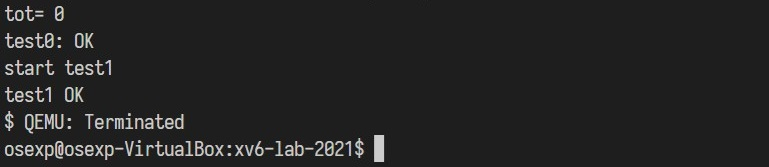
\includegraphics[width=0.8\textwidth]{lock_bcachetest.jpg}
  \caption{ \lstinline{bcachetest} 的测试结果}
\end{figure}
最后 \lstinline{bcachetest} 输出 \lstinline{test0 OK} 和 \lstinline{test1 OK},且加锁开销远小于改进前的值,符合我们的预期。

\paragraph*{实验结果} 在完成 Lab Lock 中的所有实验后,根据 MIT 6.S081 的传统,需要在实验目录下创建一个名为 \lstinline{time.txt} 文本文件,其中只包含一行,为完成该实验的小时数。然后在终端中执行 \lstinline{make grade} ,即可对整个实验进行自动评分,笔者的结果如下:
\begin{figure}[H]
  \centering
  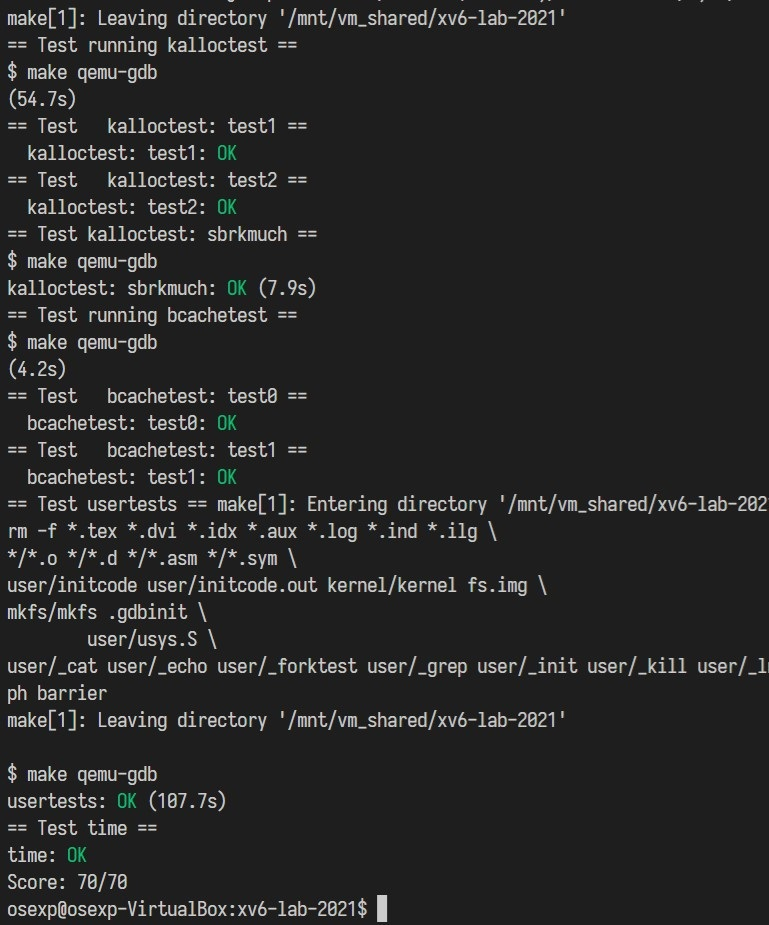
\includegraphics[width=0.5\textwidth]{lock_grade.jpg}
  \caption{ Lab Lock 的测评结果}
\end{figure}
可见测试全部通过,得分为满分。

\section{小结:减少加锁开销}

上面的两个实验很形象地展示了两种常见的减少加锁开销的方法,这里进行小结:
\begin{enumerate}
    \item 资源重复设置:在 \lstinline{kalloc} 中,通过设置多份资源以减少进程的等待概率;
    \item 细化加锁粒度:在 \lstinline{bcache} 中,通过精细化的加锁管理,减少资源加锁冲突的概率。
\end{enumerate}


